\documentclass{beamer}
\usepackage[utf8]{inputenc}

\usetheme{Madrid}
\usecolortheme{default}
\usepackage{amsmath,amssymb,amsfonts,amsthm}
\usepackage{mathtools}
\usepackage{txfonts}
\usepackage{tkz-euclide}
\usepackage{listings}
\usepackage{adjustbox}
\usepackage{array}
\usepackage{gensymb}
\usepackage{tabularx}
\usepackage{gvv}
\usepackage{lmodern}
\usepackage{circuitikz}
\usepackage{tikz}
\lstset{literate={·}{{$\cdot$}}1 {λ}{{$\lambda$}}1 {→}{{$\to$}}1}
\usepackage{graphicx}

\setbeamertemplate{page number in head/foot}[totalframenumber]

\usepackage{tcolorbox}
\tcbuselibrary{minted,breakable,xparse,skins}



\definecolor{bg}{gray}{0.95}
\DeclareTCBListing{mintedbox}{O{}m!O{}}{%
  breakable=true,
  listing engine=minted,
  listing only,
  minted language=#2,
  minted style=default,
  minted options={%
    linenos,
    gobble=0,
    breaklines=true,
    breakafter=,,
    fontsize=\small,
    numbersep=8pt,
    #1},
  boxsep=0pt,
  left skip=0pt,
  right skip=0pt,
  left=25pt,
  right=0pt,
  top=3pt,
  bottom=3pt,
  arc=5pt,
  leftrule=0pt,
  rightrule=0pt,
  bottomrule=2pt,
  toprule=2pt,
  colback=bg,
  colframe=orange!70,
  enhanced,
  overlay={%
    \begin{tcbclipinterior}
    \fill[orange!20!white] (frame.south west) rectangle ([xshift=20pt]frame.north west);
    \end{tcbclipinterior}},
  #3,
}
\lstset{
    language=C,
    basicstyle=\ttfamily\small,
    keywordstyle=\color{blue},
    stringstyle=\color{orange},
    commentstyle=\color{green!60!black},
    numbers=left,
    numberstyle=\tiny\color{gray},
    breaklines=true,
    showstringspaces=false,
}
%------------------------------------------------------------
%This block of code defines the information to appear in the
%Title page
\title %optional
{10.7.75}
\date{September 12,2025}
%\subtitle{A short story}

\author % (optional)
{Harsha-EE25BTECH11026}



\begin{document}


\frame{\titlepage}


\begin{frame}{Question}
Find the equations of tangents drawn from origin to the circle $x^2+y^2-2rx-2hy+h^2=0$,are
\begin{enumerate}
    \item $x=0$
    \item $y=0$
    \item $\brak{h^2-r^2}x-2rhy=0$
    \item $\brak{h^2-r^2}x+2rhy=0$
\end{enumerate}
\end{frame}

\begin{frame}{Theoretical Solution}
Given the equation of circle,
\begin{align}
    \vec{x}^{\top}\vec{V}\vec{x}+2\vec{u}^{\top}\vec{x}+f=0 \label{eq:1}
\end{align}
where, $\vec{x}=\myvec{x\\y}$,$\vec{V}=\myvec{1&&0\\0&&1}$,$\vec{u}=\myvec{-r\\-h}$ and $f=h^2$.\\ 
\\
It is given that the tangents pass through the origin.
\begin{align}
    \therefore \vec{n}^{\top}\vec{x}=0 \label{eq:2}
\end{align}
where $\vec{n}$ is the direction vector of the tangent.
\end{frame}

\begin{frame}{Theoretical Solution}
It is known that for any conic , the condition of tangency is given by,
\begin{align}
    \vec{n}^{\top}\vec{\Sigma}\vec{n}=0 \label{eq:3}
\end{align}
where,
\begin{align}
    \vec{n}=\myvec{1\\m}\brak{\text{Direction vector of tangent}}
\end{align}
\begin{align}
   \vec{\Sigma}=\brak{\vec{V}\vec{h}+\vec{u}}\brak{\vec{V}\vec{h}+\vec{u}}^{\top}-S\brak{\vec{h}}\vec{V} \label{eq:4}
\end{align}
$\vec{h}$ is the point through which the tangent passes and $S\brak{\vec{h}}=\vec{h}^{\top}\vec{V}\vec{h}+2\vec{u}^{\top}\vec{h}+f=0$.
\end{frame}

\begin{frame}{Theoretical Solution}
From ~\eqref{eq:2}, ~\eqref{eq:4} reduces to,
\begin{align}
    \vec{\Sigma}=\vec{u}\vec{u}^{\top}-f\vec{V}
\end{align}
yielding,
\begin{align}
    \vec{n}^{\top}\brak{\vec{u}\vec{u}^{\top}-f\vec{V}}\vec{n}=0
\end{align}
\begin{align}
    \implies \vec{n}^{\top}\vec{u}\vec{u}^{\top}\vec{n}-f\vec{n}^{\top}\vec{V}\vec{n}=0 
\end{align}
\begin{align}
    \therefore \|\vec{u}^{\top}\vec{n}\|^2=f\vec{n}^{\top}\vec{V}\vec{n} \label{eq:5}
\end{align}
\end{frame}

\begin{frame}{Theoretical Solution}
Substituting $\vec{V}$ in ~\eqref{eq:5},
\begin{align}
    \implies \|\vec{u}^{\top}\vec{n}\|^2=f\|\vec{n}\|^2
\end{align}
\begin{align}
    \implies \brak{rm+h}^2=h^2\brak{1+m^2}
\end{align}
\begin{align}
    \therefore m\brak{\brak{r^2-h^2}m-2rh}=0
\end{align}
\begin{align}
    \implies \vec{n}=\myvec{1\\0} \qquad \vec{n}=\myvec{h^2-r^2\\-2rh}
\end{align}
\end{frame}

\begin{frame}[fragile]
    \frametitle{C Code -Finding the equation of tangents}

    \begin{lstlisting}[language=C]
#include <stdio.h>

void solve_tangents(double r, double h, double tangents[4]) {
    // First tangent: x = 0 -> line (1,0)
    tangents[0] = 1.0;
    tangents[1] = 0.0;
    // Second tangent: (h^2 - r^2)x - 2rh y = 0
    double a = h*h - r*r;
    double b = -2.0*r*h;

    if (a == 0 && b == 0) {
        // Special case -> y=0
        tangents[2] = 0.0;
        tangents[3] = 1.0;
    } else {
        tangents[2] = a;
        tangents[3] = b;
    }
}
    \end{lstlisting}
\end{frame}


\begin{frame}[fragile]
    \frametitle{Python+C code}

    \begin{lstlisting}[language=Python]
import ctypes
import numpy as np
import matplotlib.pyplot as plt

# Load shared C library
lib = ctypes.CDLL("./libtangent_solver.so")

# Define C function signature
lib.solve_tangents.argtypes = [ctypes.c_double, ctypes.c_double,
                               ctypes.POINTER(ctypes.c_double)]
lib.solve_tangents.restype = None

def get_tangents_from_c(r, h):
    results = (ctypes.c_double * 4)()
    lib.solve_tangents(r, h, results)
    vals = list(results)
    tangents = [(vals[0], vals[1]), (vals[2], vals[3])]
    \end{lstlisting}
\end{frame}

\begin{frame}[fragile]
    \frametitle{Python+C code}

    \begin{lstlisting}[language=Python]
 tangent_eqs = []
    for a, b in tangents:
        if b == 0:  # x=0
            tangent_eqs.append("x = 0")
        elif a == 0:  # y=0
            tangent_eqs.append("y = 0")
        else:
            tangent_eqs.append(f"{a:.0f}x {b:+.0f}y = 0")

    return tangents, tangent_eqs

def plot_tangents(r, h):
    tangents, tangent_eqs = get_tangents_from_c(r, h)

    print("Tangents from origin:")
    for eq in tangent_eqs:
        print("   ", eq)
    \end{lstlisting}
\end{frame}

\begin{frame}[fragile]
    \frametitle{Python+C code}

    \begin{lstlisting}[language=Python]
 # Circle
    theta = np.linspace(0, 2*np.pi, 400)
    x_circ = r + r*np.cos(theta)
    y_circ = h + r*np.sin(theta)

    plt.figure(figsize=(6,6))
    plt.plot(x_circ, y_circ, 'b', label="Circle")

    # Tangents
    x_vals = np.linspace(-2*r, 2*r, 400)
    for (a,b), eq in zip(tangents, tangent_eqs):
        if b == 0:
            plt.axvline(0, color='r', linestyle='--', label=eq)
        else:
            y_vals = -(a/b)*x_vals
            plt.plot(x_vals, y_vals, 'r--', label=eq)
    \end{lstlisting}
\end{frame}

\begin{frame}[fragile]
    \frametitle{Python+C code}

    \begin{lstlisting}[language=Python]
# Origin & center
    plt.scatter([0],[0], color='k', marker='o', label="Origin (0,0)")
    plt.scatter([r],[h], color='g', marker='x', label=f"Center ({r},{h})")

    plt.gca().set_aspect('equal', adjustable='box')
    plt.axhline(0, color='gray', linewidth=0.5)
    plt.axvline(0, color='gray', linewidth=0.5)
    plt.legend()
    plt.title(f"Tangents from Origin to Circle (r={r}, h={h})")
    plt.savefig("/home/user/Matrix Theory: workspace/Matgeo_assignments/10.7.75/figs/figure_1.png")
    plt.show()

# Example
plot_tangents(r=3, h=4)


    \end{lstlisting}
\end{frame}

\begin{frame}[fragile]
    \frametitle{Python code}
    \begin{lstlisting}[language=Python]
import numpy as np
import matplotlib.pyplot as plt

def tangents_from_origin(r, h):
    """
    Finds tangent lines from origin to the circle
    x^2 + y^2 - 2rx - 2hy + h^2 = 0.
    
    Returns:
        tangents: list of (a,b) representing ax+by=0
        tangent_eqs: list of pretty string equations
    """
    tangents = []
    tangent_eqs = []
    # Case 1: x=0
    tangents.append((1, 0))
    tangent_eqs.append("x = 0")

    \end{lstlisting}   
\end{frame}

\begin{frame}[fragile]
    \frametitle{Python code}
    \begin{lstlisting}[language=Python]
# Case 2
    if (h**2 - r**2) != 0:
        a, b = (h**2 - r**2, -2*r*h)
        tangents.append((a, b))
        tangent_eqs.append(f"{a}x {b:+}y = 0")
    else:
        tangents.append((0, 1))
        tangent_eqs.append("y = 0")
        
    return tangents, tangent_eqs

def plot_tangents(r, h):
    tangents, tangent_eqs = tangents_from_origin(r, h)
    
    # Print immediately
    print("Tangents from origin:")
    for eq in tangent_eqs:
        print("   ", eq)
    \end{lstlisting}   
\end{frame}

\begin{frame}[fragile]
    \frametitle{Python code}
    \begin{lstlisting}[language=Python]
# Circle: center = (r,h), radius = r
    theta = np.linspace(0, 2*np.pi, 400)
    x_circ = r + r*np.cos(theta)
    y_circ = h + r*np.sin(theta)

    plt.figure(figsize=(6,6))
    plt.plot(x_circ, y_circ, 'b', label="Circle")

    # Tangents
    x_vals = np.linspace(-2*r, 2*r, 400)
    for (a,b), eq in zip(tangents, tangent_eqs):
        if b == 0:
            plt.axvline(0, color='r', linestyle='--', label=eq)
        else:
            y_vals = -(a/b)*x_vals
            plt.plot(x_vals, y_vals, 'r--', label=eq)
    \end{lstlisting}   
\end{frame}

\begin{frame}[fragile]
    \frametitle{Python code}
    \begin{lstlisting}[language=Python]
# Mark origin & center
    plt.scatter([0],[0], color='k', marker='o', label="Origin (0,0)")
    plt.scatter([r],[h], color='g', marker='x', label=f"Center ({r},{h})")

    plt.gca().set_aspect('equal', adjustable='box')
    plt.axhline(0, color='gray', linewidth=0.5)
    plt.axvline(0, color='gray', linewidth=0.5)
    plt.legend()
    plt.title(f"Tangents from Origin to Circle (r={r}, h={h})")
    plt.savefig("/home/user/Matrix Theory: workspace/Matgeo_assignments/10.7.75/figs/Figure_1.png")
    plt.show()

# Example usage
plot_tangents(r=3, h=4)
    \end{lstlisting}   
\end{frame}

\begin{frame}{Plot}
    \begin{figure}[H]
    \centering
    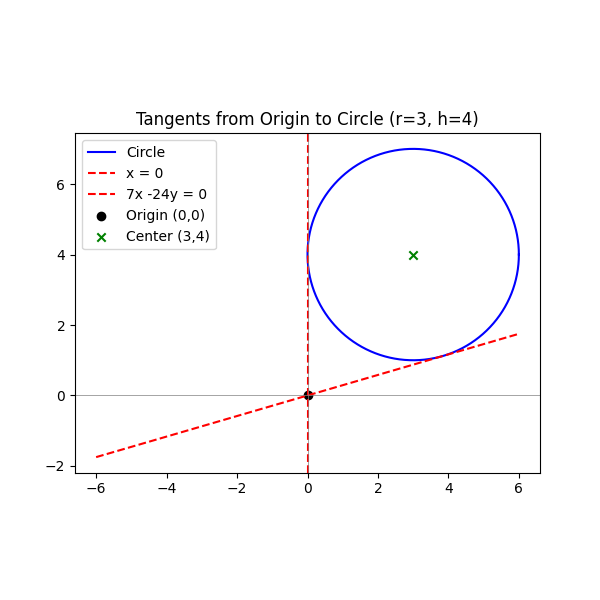
\includegraphics[width=0.6\columnwidth]{figs/Figure_1.png}
    \label{fig:1}
    \end{figure}
\end{frame}

\end{document}